\documentclass[12pt]{article}
\usepackage[english]{babel}
\usepackage[letterpaper,margin=1in]{geometry}
\usepackage[parfill]{parskip}
\usepackage{graphicx}
\usepackage{mathtools}
\usepackage{amssymb}
\graphicspath{{img/}}
\usepackage{hyperref}
\frenchspacing
\author{Ariel Davis (azdavis), Jerry Yu (jerryy)}
\date{\today}
\title{15-418 Final Project Report}
\begin{document}
\maketitle

Repo: \url{https://github.com/azdavis/parallel-portrait-mode}

\section{Overview}

We implemented portrait mode in parallel. Portrait mode has traditionally been
done by high end DSLR camera hardware, which the foreground of the subject is
in focus and the background is blurred. We have chosen to use a software-only
image processing approach to this problem, segmenting the image into the
foreground and blurring the background.

On our largest images, we were able to achieve 150x speedup with CUDA on GPUs
and 11x speedup with OpenMP on CPUs.

\begin{figure}[!htb]
    \begin{minipage}{0.48\textwidth}
        \centering
        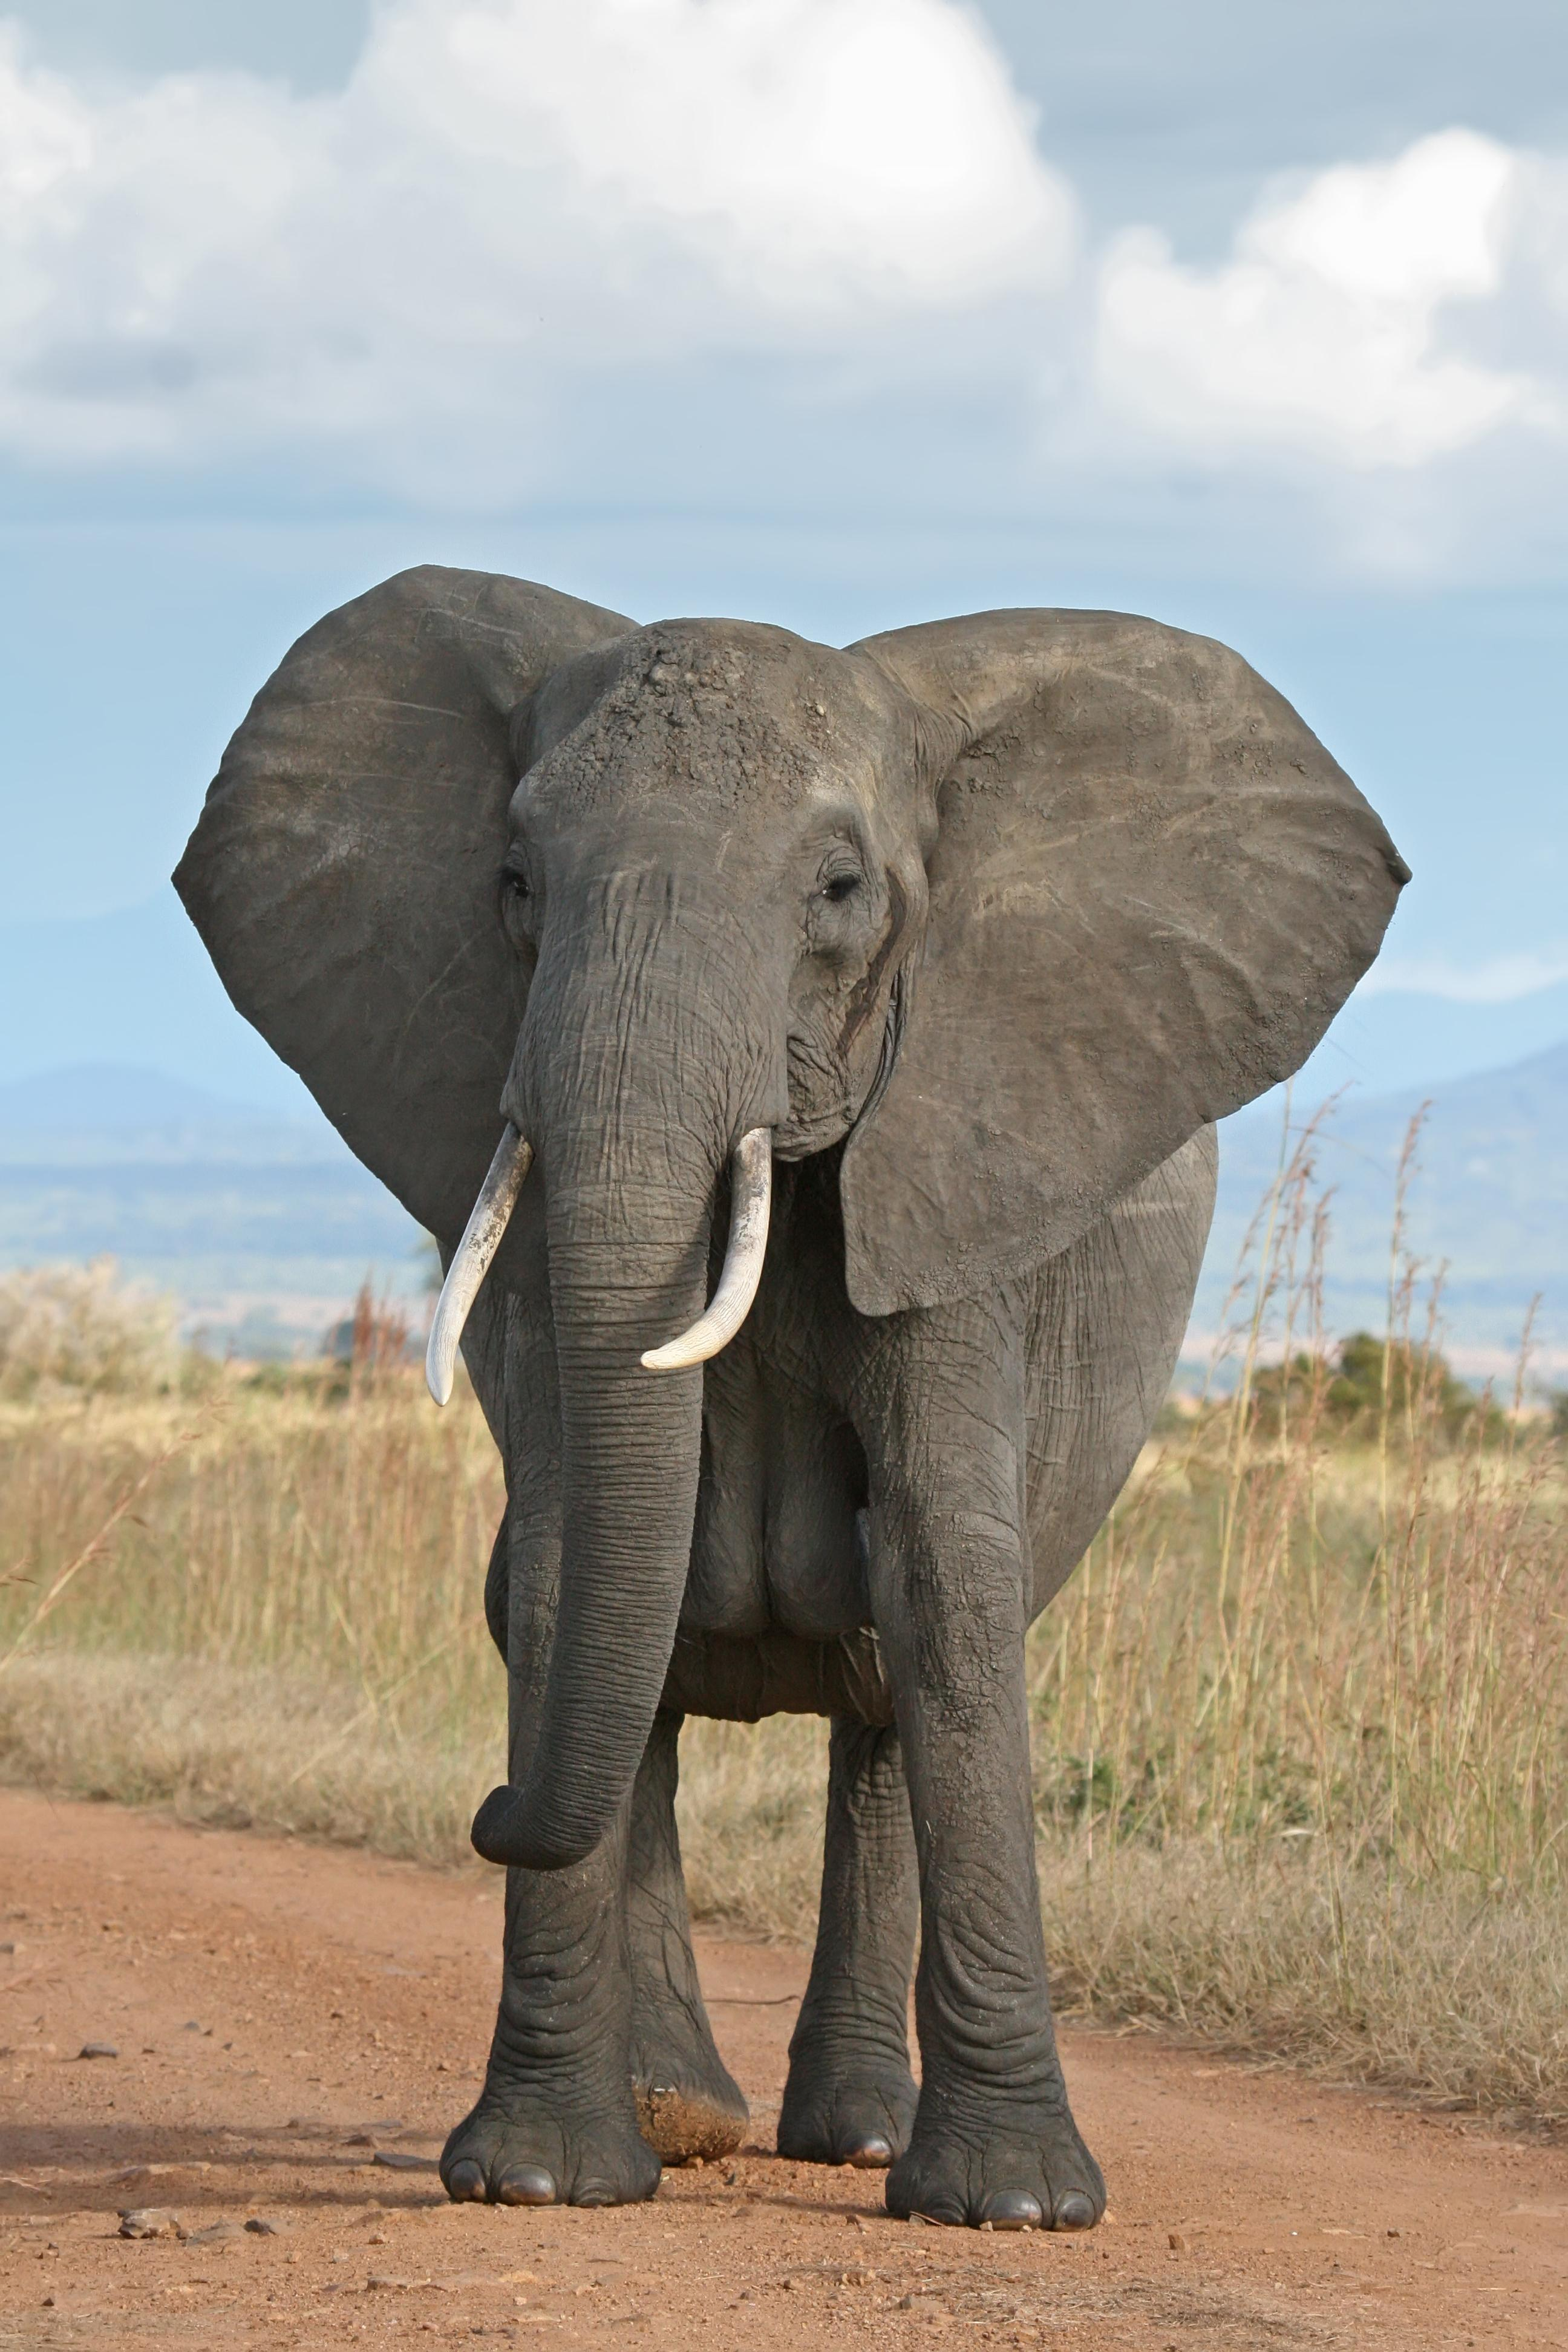
\includegraphics[width=0.9\linewidth]{large_elephant.jpg}
        \caption{Input Image}
    \end{minipage}\hfill
    \begin{minipage}{0.48\textwidth}
        \centering
        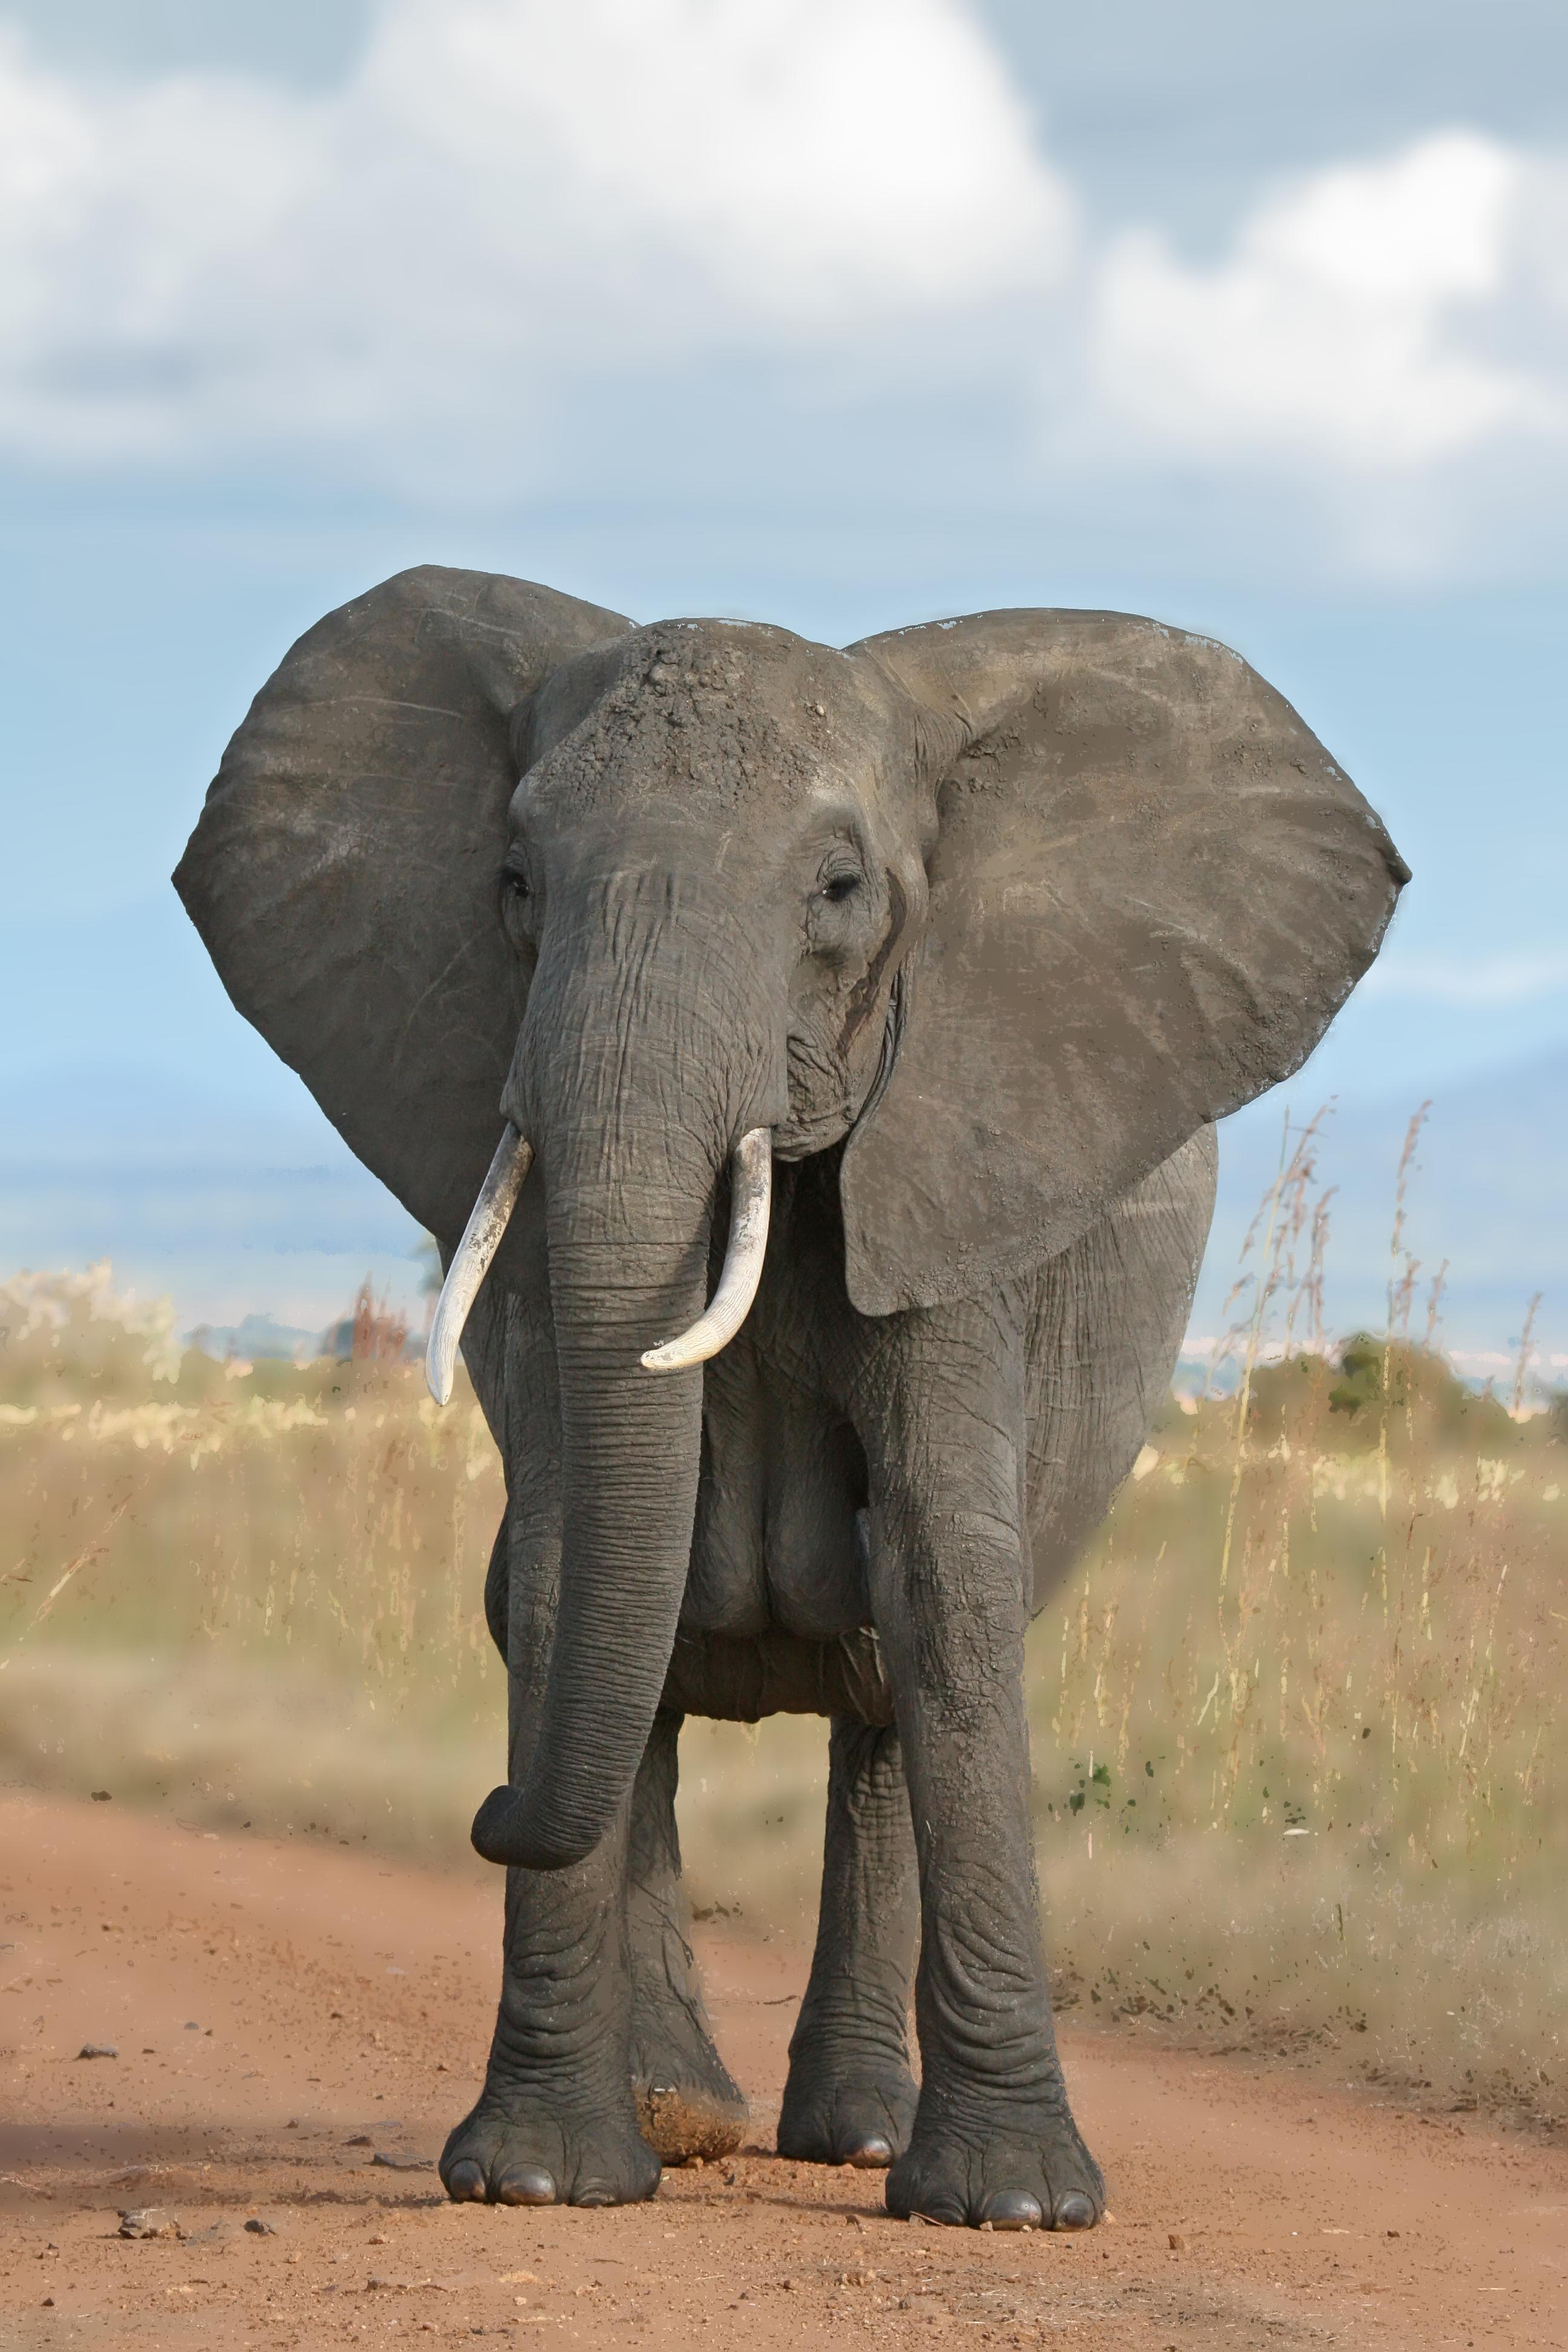
\includegraphics[width=0.9\linewidth]{large_elephant_portrait.jpg}
        \caption{Output Portrait Mode Image}
    \end{minipage}\hfill
\end{figure}

\section{Algorithm}

We used a simplified version of the grab-cut algorithm, with the idea of
getting the color distribution of the background to find the foreground. Our
algorithm takes in input image and returns the image in portrait mode.

Each step of the algorithm will be referred to its shortened name in
parenthesis.

\begin{enumerate}
    \item
        Designiate the borders of the image as the background. Top, left, and
        right $\tfrac{1}{8}$ of image.
    \item
        Get a color distribution of the background region. For each background
        pixel, increment the appropriate color count bucket. (Color Counts)
    \item
        Create a foreground mask by finding every pixel with a color not
        in the background color distribution. Filter background colors that
        make up less than 1 percent of the background area. (Build Mask)
    \item
        For every unmasked pixel, add it to the mask if two of its neighboring
        pixels were part of the mask. (Refine Mask)
    \item
        Blur all the pixels that are not within the foreground mask. We used a
        convolution with a circular filter to emulate the bokeh effect. (Blur)
    \item
        For each pixel in the mask, add the original pixel of the image into
        the blurred version of the image.
\end{enumerate}

\begin{figure}[!htb]
    \begin{minipage}{0.48\textwidth}
        \centering
        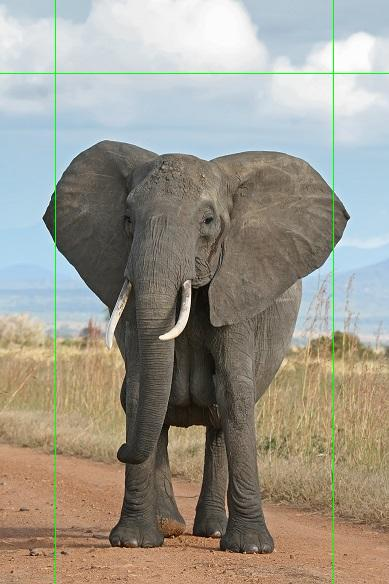
\includegraphics[width=0.5\linewidth]{border.jpg}
        \caption{Background Region (Step 1)}
    \end{minipage}\hfill
    \begin{minipage}{0.48\textwidth}
        \centering
        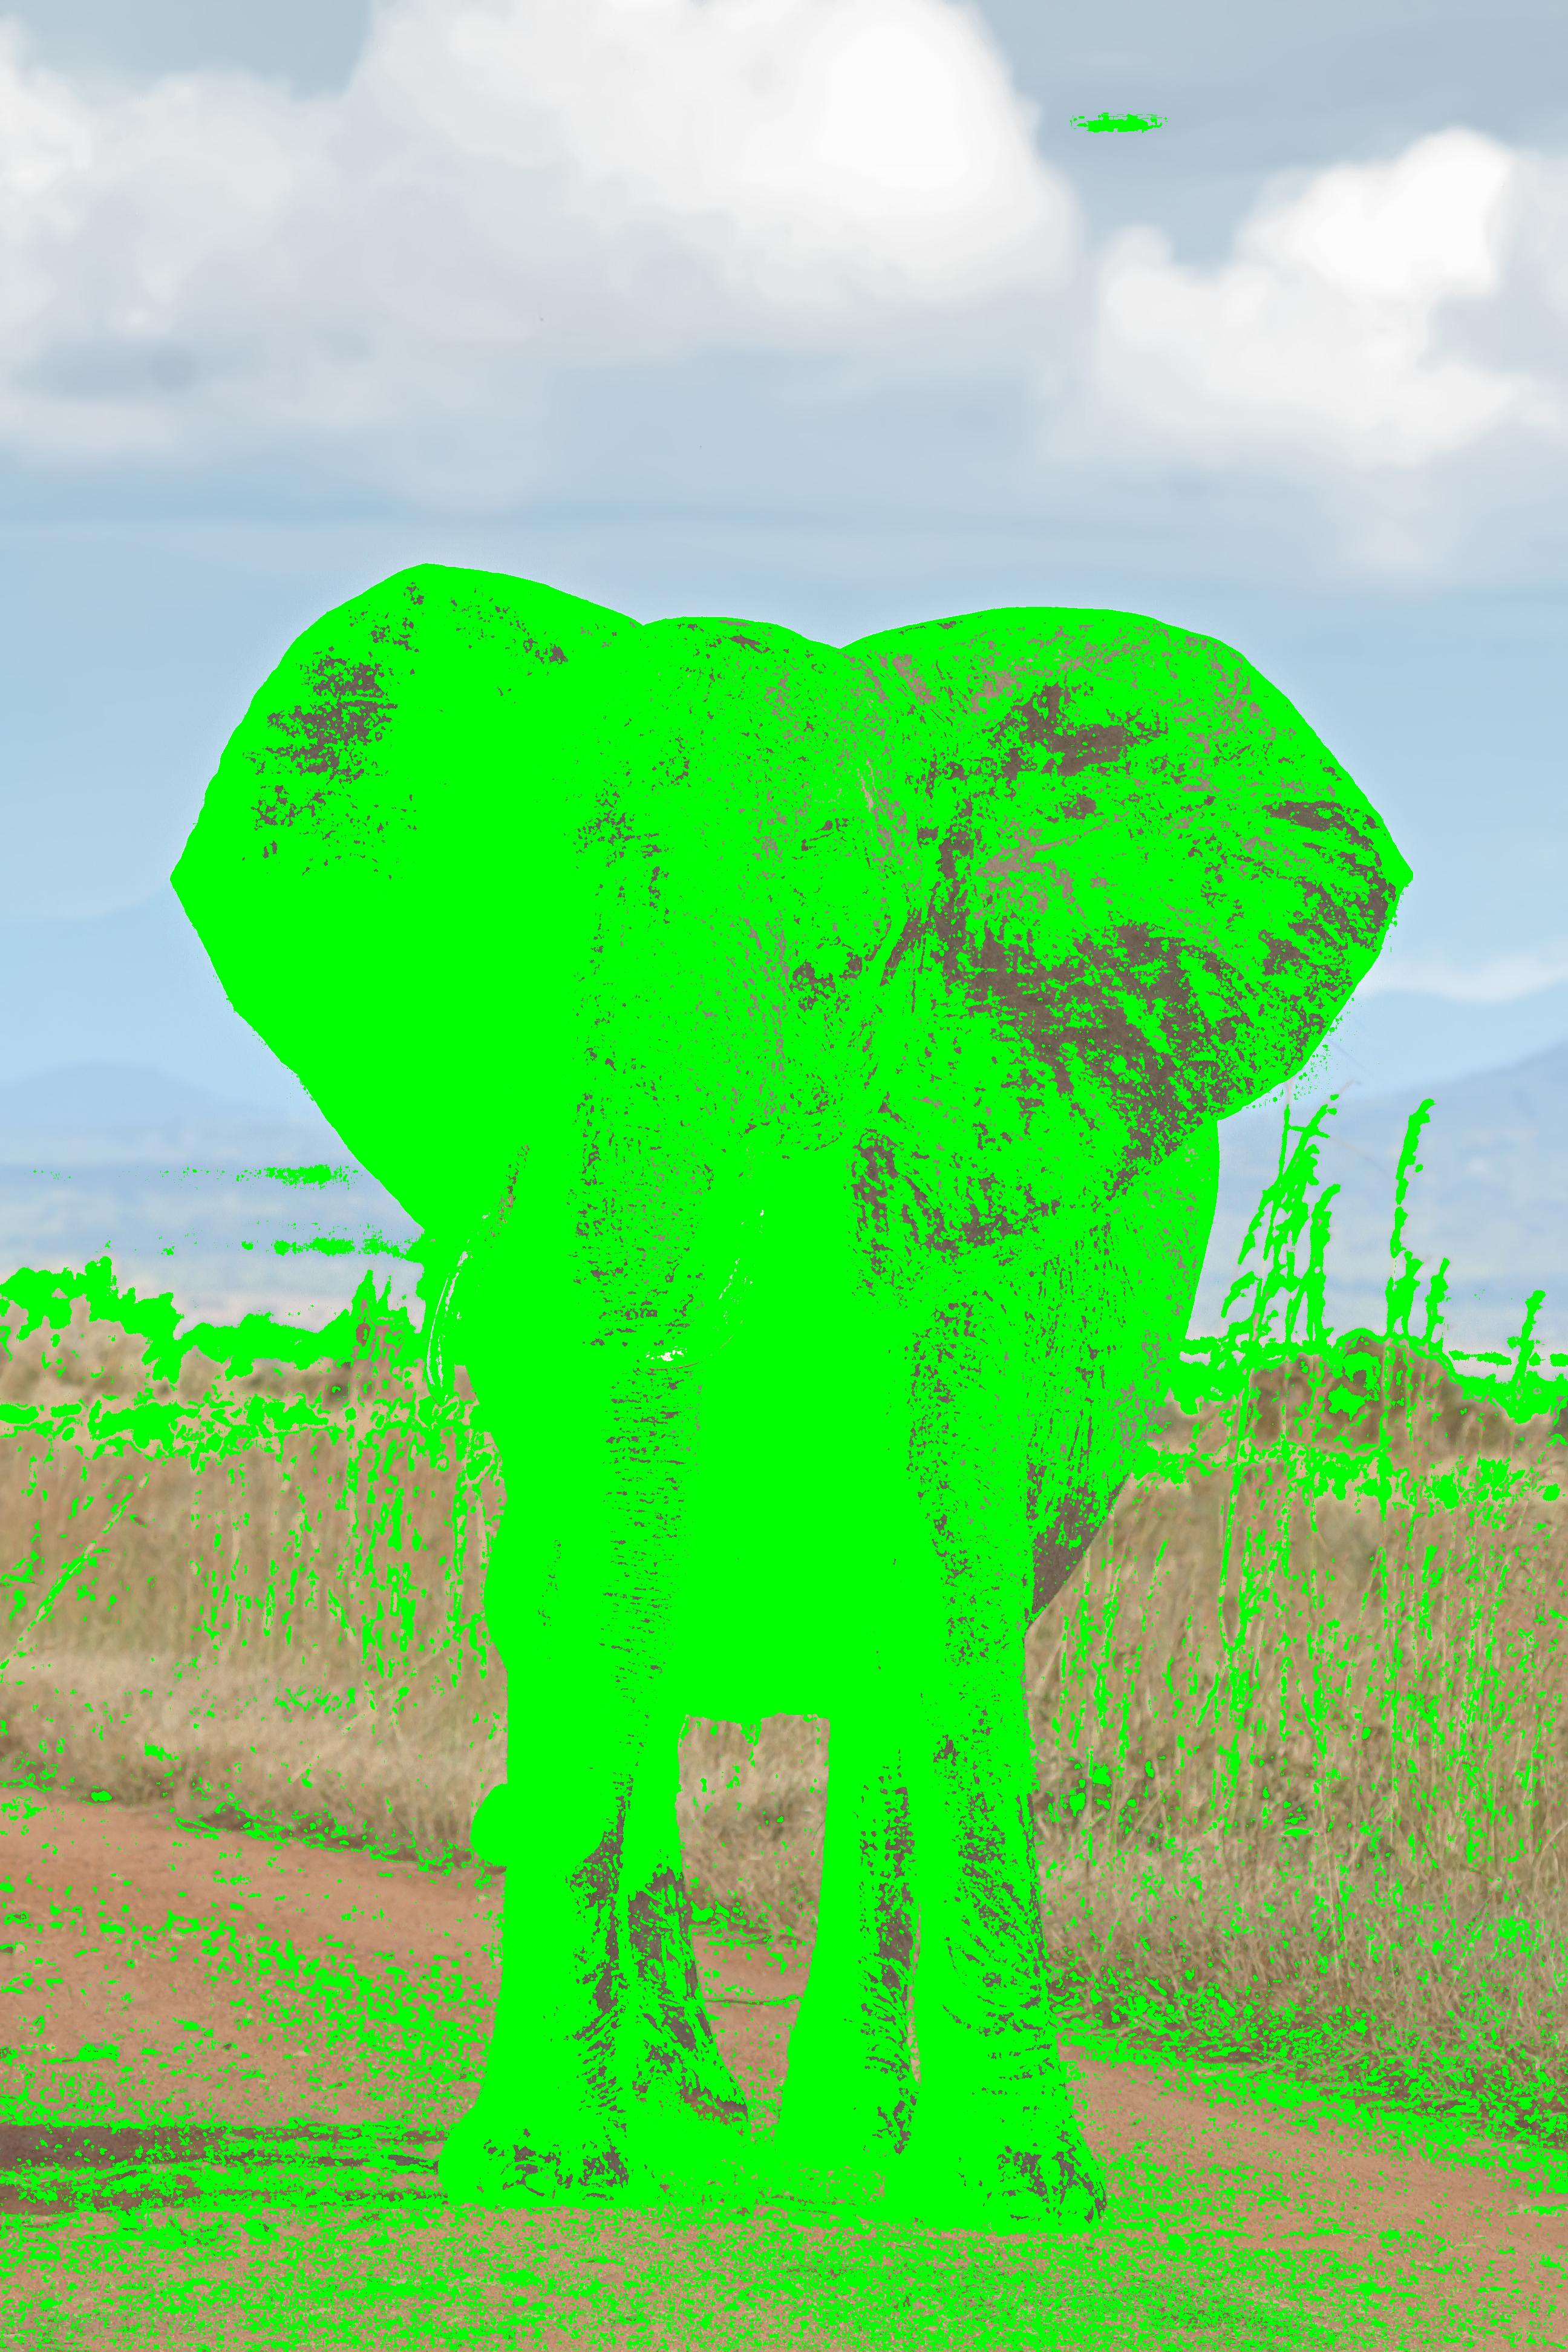
\includegraphics[width=0.5\linewidth]{mask.jpg}
        \caption{Foreground Mask (Step 5)}
    \end{minipage}\hfill
\end{figure}

\subsection{Data Structures}

Each image is represented as a struct with the width, height, and an array of
pixels. Each pixel contains a red, green, and blue value. The size of the array
is the number of pixels in the image.

We stored the color counts by creating color buckets for every RGB value.
Essentially, all colors in one bucket would be within 15 red, green, and blue
value. This results in $\left(\tfrac{255}{15}\right)^3$ different buckets. So,
we are able to store the color counts with an array, with each element
representing the count for that bucket.

The mask is simply an array of chars the size of the number of pixels in the
image. If the value in the mask is 1, the corresponding pixel is in the
foreground. Otherwise, it is in the background. We chose chars to minimize the
size of the data structure.

\subsection{Background}

The blur is the most computationally intensive part of the algorithm. Each
pixel of the blurred image needs to compute the average RGB values for a circle
of pixels around it. However, the blur is data parallel, as each pixel is
independent.

However, each step of the algorithm has to be finished before the next step.
This requires synchronization after each step.

\section{Approach}

We were interested in comparing the GPU and CPU implementations of our
algorithm, so we implemented it in CUDA and OpenMP. To develop and solidify our
algorithm, we first wrote an implementation with Python's NumPy before moving
on to sequential C and then parallelism. We experimented with several edge
detection, gradient, and snake methods and decided the color distribution
method gave us the best accuracy for foreground detection.

\section{CUDA on GPU}

We utilized the NVIDIA 1080x GPUs in the Gates Clusters with CUDA. The general
strategy for CUDA was to parallelize across the pixels in the image to take
advantage of the high number of ALUs and threads.

\subsection{Color Counts}

To get the color counts, we assigned each thread to each pixel. Each thread
then did an atomic add to appropriate bucket in color counts. An atomic add was
needed because multiple pixels could simultaneously have the same color.

We also tried assigning one thread to one color to iterate through the image,
but that was repeating the sequential algorithm of looking at each pixel.

Another implementation was to create copies of the color counts data structure
for each thread to process, but one of our timing bottlenecks was performing
cudaMallocs to initialize memory in CUDA. (discussed later on)

So, we moved forward with the atomic strategy. We initially thought the
contention all the threads would slow this part of the algorithm, but our
timing showed us atomic allowed this step to be performed in almost 0 time.

\subsection{Build Mask and Refine Mask}

The CUDA implementation of build mask and refine mask were more straight
forward. Each thread was simply mapped to one pixel.

We tried to compute both steps within one launch, but realized we needed to
synchronize or communicate between warps. The overhead of another launch was
less, so we just kept the two steps in two launches.

\subsection{Blur}

We were able to take advantage of the data parallelism for the blur, as each
pixel's computation was indepedent from those of other pixels. So, each pixel
is mapped to one CUDA thread. Additionally, pixels spatially close are mapped
to the same block. This allowed us to take advantage of the high amount of
threads in each SM. This mapping significantly decreased the arithmetic
computation per thread, but we realized that we had a memory bottleneck.

We noticed that the pixels close together needed to access the same neighboring
pixels to perform the convolution. So, we loaded every pixel needed for that
block's blur into shared memory. The kernel that contained the weights for how
much each neighboring pixel contributed to the average was also loaded into
shared memory. By having each thread load data into shared memory, the cost of
loading it is very low while allowing every memory access to be from shared
memory.

\begin{center}
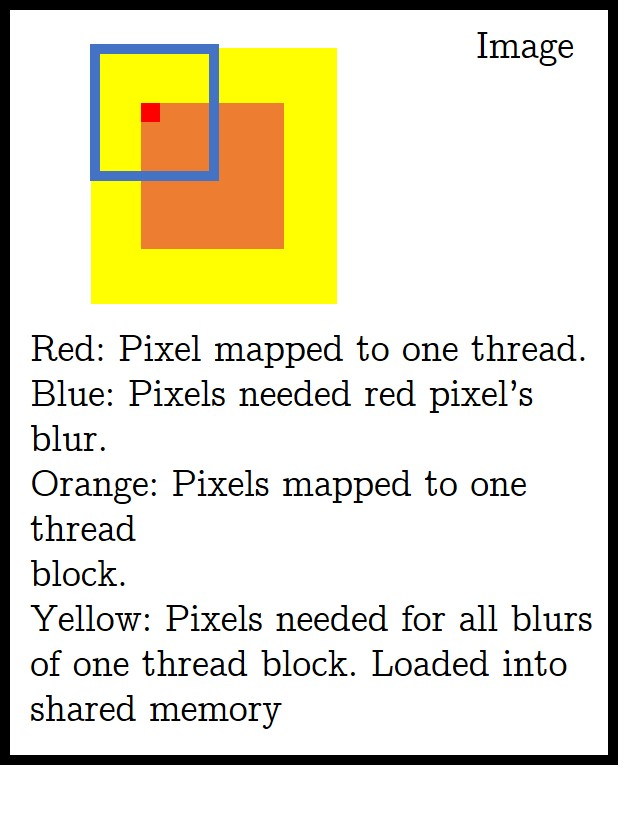
\includegraphics[scale=0.3]{mapping.jpg} \\
Thread mapping and shared memory for CUDA blur
\end{center}

\section{OpenMP on CPU}

We utilized the 16 core CPUs in the Gates Clusters with OpenMP. For CPUs, there
was not enough threads to parallelize across every pixel like on GPUs. So, we
chose to parallelize across rows of the image, keeping arithmetic intensity
high while using parallelism.

\subsection{Color Counts}

We chose not to parallelize the color counts step in our algorithm. From our
profiling, getting the color counts made up less than 0.03 percent of our time,
and that overhead with parallelism would not increase our speedup.

We first tried the atomic strategy we used for CUDA. Each thread was assigned a
row and performed an atomic add to a color bucket for each background pixel.
However, the overhead from gaining exclusive control to the bucket made the
implementation around 2x slower than sequential. For large elephant, sequential
was around 0.038s and with atomic parallel it was 0.95s.

Additional methods would be to create local copies of the data structures for
each thread and combining them in parallel.

\subsection{Build Mask and Refine Mask}

We parallelized building and refining the mask by parallelizing over the rows
of the image. We chose rows because it gave us enough arithmetic computation
while still giving us the granularity we needed for the computation.

We experimented with using SIMD in the inner loop over each column, but that
was around 1.5x slower than without SIMD. This is probably because there is an
uneven workload in one row. Each loop iteration only writes to an array if
there is a conditional, so there is uneven work that causes SIMD to take
longer.

\subsection{Blur}

Similar to the previous steps, we parallelized over the rows for the blur.
However, the work of each row varied significantly. This is because rows with
pixels in the foreground are not blurred, saving $50^2$ computations with a
filter size of 50. So, we used dyanamic scheduling with OpenMP in order to
distribute the work evenly. With parallelizing over rows and dynamic
scheduling, we were able to maintain a small granularity while still having
even work among the threads. With dynamic over static scheduling we were able
to achieve around 50 percent speedup for blur on large images. (From 15s to
10s)

We also tried adjusting the chunk size with dynamic scheduling in order to
reduce the amount of overhead with scheduling the work. However, changing the
chunk size to 5 or 10 did not increase the speed. Increasing chunk size only
increased the time differences between threads. We also experimented with using
SIMD over the columns for the inner loop of the blur. However, this resulted in
a blur that was around the same time as without SIMD. This is because new
colors for each pixel were not adjacent in memory and required scatter
operations to write to them. Many of the memory accesses also required gather
operations, which slowed down the vectorization speedups from SIMD.

\section{Results}

\subsection{Total}
\begin{tabular}{r|r|r|r|r|r|r|r|r}
    Image & Size & C++ & OMP & Speedup & CUDA & Speedup & ISPC & Speedup
\\  \hline
    Elephant & $389 \times 584$ & 2.4544 & 0.1870 & 13.1262 & 0.1267 & 19.3729 & 0.2098 & 11.6998
\\  Bluejay & $1200 \times 832$ & 13.8076 & 1.0352 & 13.3381 & 0.1424 & 96.9920 & 1.1700 & 11.8011
\\  Tiger & $1400 \times 845$ & 14.7907 & 1.3724 & 10.7769 & 0.1601 & 92.3965 & 1.5323 & 9.6524
\\  Flower & $2242 \times 2112$ & 72.4220 & 5.9389 & 12.1945 & 0.2328 & 311.1581 & 6.0131 & 12.0441
\\  Purp & $2944 \times 2609$ & 89.1033 & 7.5531 & 11.7969 & 0.2529 & 352.3457 & 7.5378 & 11.8208
\\  Large Elephant & $2592 \times 3888$ & 112.9916 & 9.5302 & 11.8562 & 0.3248 & 347.8504 & 10.5817 & 10.6780
\end{tabular}

\begin{center}
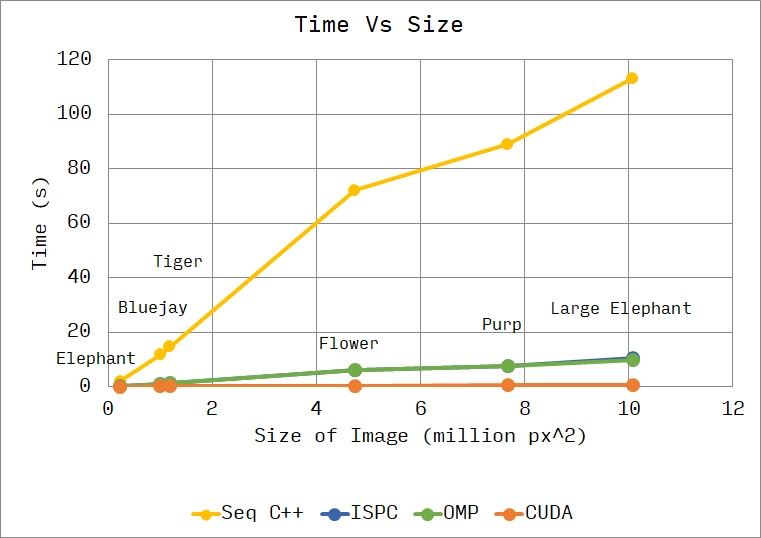
\includegraphics[scale=1]{time.jpg}
\end{center}

\begin{center}
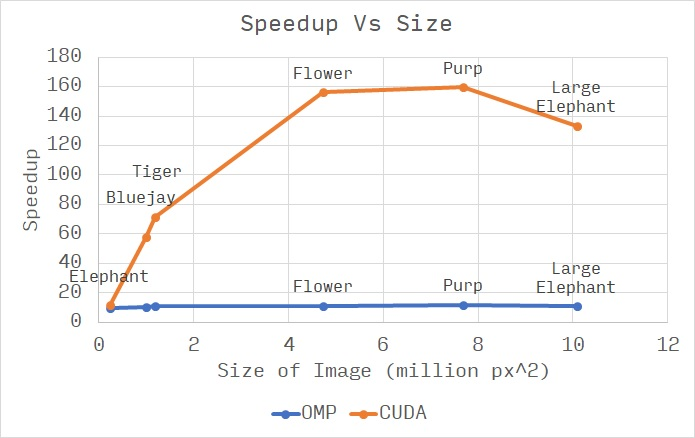
\includegraphics[scale=1]{speedup.jpg}
\end{center}

\subsection{Elephant ($\mathbf{389 \times 584}$ px)}

\begin{tabular}{r|r|r|r|r|r|r|r}
    Item & C++ & OMP & Speedup & CUDA & Speedup & ISPC & Speedup
\\  \hline
    init & 0.0006 & 0.0004 & 1.5932 & 0.1213 & 0.0046 & 0.0003 & 1.6686
\\  color counts & 0.0006 & 0.0003 & 2.0066 & 0.0000 & 17.9412 & 0.0003 & 2.0539
\\  build mask & 0.0016 & 0.0003 & 5.1911 & 0.0001 & 16.6327 & 0.0004 & 4.4780
\\  refine mask & 0.0010 & 0.0002 & 4.3612 & 0.0000 & 76.1538 & 0.0002 & 4.4000
\\  blur & 2.4503 & 0.1856 & 13.1990 & 0.0049 & 503.9673 & 0.2084 & 11.7565
\\  clean up & 0.0003 & 0.0001 & 1.9433 & 0.0003 & 0.8035 & 0.0001 & 2.0602
\\  \hline
    total & 2.4544 & 0.1870 & 13.1262 & 0.1267 & 19.3729 & 0.2098 & 11.6998
\end{tabular}

\subsection{Bluejay ($\mathbf{1200 \times 832}$ px)}

\begin{tabular}{r|r|r|r|r|r|r|r}
    Item & C++ & OMP & Speedup & CUDA & Speedup & ISPC & Speedup
\\  \hline
    init & 0.0019 & 0.0007 & 2.6037 & 0.1199 & 0.0162 & 0.0012 & 1.6667
\\  color counts & 0.0029 & 0.0013 & 2.3474 & 0.0000 & 86.6471 & 0.0012 & 2.4227
\\  build mask & 0.0075 & 0.0007 & 10.6453 & 0.0003 & 23.2804 & 0.0007 & 10.6910
\\  refine mask & 0.0051 & 0.0009 & 5.4111 & 0.0000 & 390.8462 & 0.0009 & 5.4053
\\  blur & 13.7894 & 1.0312 & 13.3723 & 0.0217 & 635.0481 & 1.1655 & 11.8310
\\  clean up & 0.0007 & 0.0004 & 1.9586 & 0.0004 & 1.7904 & 0.0005 & 1.5085
\\  \hline
    total & 13.8076 & 1.0352 & 13.3381 & 0.1424 & 96.9920 & 1.1700 & 11.8011
\end{tabular}

\subsection{Tiger ($\mathbf{1400 \times 845}$ px)}

\begin{tabular}{r|r|r|r|r|r|r|r}
    Item & C++ & OMP & Speedup & CUDA & Speedup & ISPC & Speedup
\\  \hline
    init & 0.0015 & 0.0011 & 1.3638 & 0.1352 & 0.0110 & 0.0015 & 0.9987
\\  color counts & 0.0019 & 0.0015 & 1.2468 & 0.0000 & 44.5000 & 0.0014 & 1.3033
\\  build mask & 0.0060 & 0.0043 & 1.3867 & 0.0003 & 17.6374 & 0.0009 & 6.9896
\\  refine mask & 0.0043 & 0.0043 & 0.9917 & 0.0000 & 268.0625 & 0.0011 & 3.7557
\\  blur & 14.7767 & 1.3606 & 10.8601 & 0.0237 & 624.4102 & 1.5269 & 9.6776
\\  clean up & 0.0004 & 0.0005 & 0.7148 & 0.0008 & 0.4700 & 0.0005 & 0.7637
\\  \hline
    total & 14.7907 & 1.3724 & 10.7769 & 0.1601 & 92.3965 & 1.5323 & 9.6524
\end{tabular}

\subsection{Flower ($\mathbf{2242 \times 2112}$ px)}

\begin{tabular}{r|r|r|r|r|r|r|r}
    Item & C++ & OMP & Speedup & CUDA & Speedup & ISPC & Speedup
\\  \hline
    init & 0.0062 & 0.0047 & 1.3030 & 0.1437 & 0.0430 & 0.0038 & 1.6386
\\  color counts & 0.0185 & 0.0061 & 3.0178 & 0.0000 & 499.0000 & 0.0058 & 3.1866
\\  build mask & 0.0397 & 0.0029 & 13.8337 & 0.0012 & 34.1731 & 0.0024 & 16.2469
\\  refine mask & 0.0197 & 0.0067 & 2.9648 & 0.0000 & 1096.1667 & 0.0038 & 5.2476
\\  blur & 72.3376 & 5.9179 & 12.2236 & 0.0867 & 834.7293 & 5.9969 & 12.0625
\\  clean up & 0.0004 & 0.0007 & 0.5299 & 0.0012 & 0.2921 & 0.0004 & 0.8698
\\  \hline
    total & 72.4220 & 5.9389 & 12.1945 & 0.2328 & 311.1581 & 6.0131 & 12.0441
\end{tabular}

\subsection{Purp ($\mathbf{2944 \times 2609}$ px)}

\begin{tabular}{r|r|r|r|r|r|r|r}
    Item & C++ & OMP & Speedup & CUDA & Speedup & ISPC & Speedup
\\  \hline
    init & 0.0058 & 0.0059 & 0.9986 & 0.1352 & 0.0432 & 0.0059 & 0.9892
\\  color counts & 0.0125 & 0.0100 & 1.2482 & 0.0000 & 304.2683 & 0.0096 & 1.2948
\\  build mask & 0.0301 & 0.0088 & 3.4112 & 0.0016 & 18.5774 & 0.0090 & 3.3386
\\  refine mask & 0.0160 & 0.0073 & 2.1746 & 0.0000 & 887.2222 & 0.0077 & 2.0646
\\  blur & 89.0385 & 7.5199 & 11.8404 & 0.1145 & 777.7034 & 7.5049 & 11.8640
\\  clean up & 0.0004 & 0.0012 & 0.3377 & 0.0015 & 0.2784 & 0.0006 & 0.6810
\\  \hline
    total & 89.1033 & 7.5531 & 11.7969 & 0.2529 & 352.3457 & 7.5378 & 11.8208
\end{tabular}

\subsection{Large Elephant ($\mathbf{2592 \times 3888}$ px)}

\begin{tabular}{r|r|r|r|r|r|r|r}
    Item & C++ & OMP & Speedup & CUDA & Speedup & ISPC & Speedup
\\  \hline
    init & 0.0075 & 0.0077 & 0.9830 & 0.1505 & 0.0500 & 0.0077 & 0.9812
\\  color counts & 0.0164 & 0.0130 & 1.2582 & 0.0000 & 389.9524 & 0.0123 & 1.3270
\\  build mask & 0.0464 & 0.0058 & 8.0007 & 0.0026 & 17.6362 & 0.0058 & 8.0381
\\  refine mask & 0.0295 & 0.0085 & 3.4814 & 0.0000 & 1638.5556 & 0.0081 & 3.6242
\\  blur & 112.8914 & 9.4943 & 11.8904 & 0.1700 & 663.8989 & 10.5470 & 10.7036
\\  clean up & 0.0004 & 0.0009 & 0.4150 & 0.0016 & 0.2265 & 0.0007 & 0.5007
\\  \hline
    total & 112.9916 & 9.5302 & 11.8562 & 0.3248 & 347.8504 & 10.5817 & 10.6780
\end{tabular}

\end{document}
